\lstdefinelanguage{plaintext}{
  sensitive=false,
  comment=[l]{//},
  morecomment=[s]{/*}{*/},
  identifierstyle=\color{black},
  morestring=[b]',
  morestring=[b]"
}

\lstset
{ 
    language=plaintext,
    basicstyle=\footnotesize,
    numbers=left,
    stepnumber=1,
    showstringspaces=false,
    tabsize=1,
    breaklines=true,
    breakatwhitespace=false,
    frame=leftline
}

\chapter{Analisis dan Perancangan Perangkat Lunak}
\label{chap:Perancangan}

Pada bab ini dibahas mengenai perancangan perangkat lunak yang dibangun, meliputi perancangan kelas dan algoritma pengecekan dokumen skripsi.

\section{Perancangan Metode Pemeriksaan}
Pada bagian ini akan dijelaskan rancangan metode yang akan digunakan oleh setiap fitur pemeriksaan. Pemeriksaan kesalahan dokumen skripsi akan menggunakan metode pencocokan pola. Pola tersebut akan dibuat dengan menggunakan \textit{regular expression}. Setiap fitur memiliki pola yang berbeda, sesuai dengan fungsi yang dimiliki oleh masing-masing fitur. Berikut ini akan dijelaskan pola-pola yang akan digunakan:

\begin{itemize}
	\item Fitur PS-01 \newline
	Pada fitur ini, pemeriksaan dilakukan dengan cara membandingkan kata-kata yang ada pada dokumen dengan kata-kata yang ada pada kamus. Kode imbuhan yang ada pada kamus dihilangkan dengan menggunakan regular expression. Hal ini dilakukan karena pemeriksaan kata mengabaikan imbuhan yang ada pada kamus.
	
	\item Fitur PS-03 \newline
	Pada fitur ini, pemeriksaan dilakukan dengan cara mencari pola kalimat yang penulisan tanda bacanya berhimpitan antara 2 kata. Selain itu tanda baca titik pada akhir kalimat yang berhimpitan dengan kata pertama pada kalimat baru. Pola \textit{regular expression} yang digunakan akan diuraikan pada Listing \ref{lst:ps03}.
	
\begin{lstlisting}[caption={Pola \textit{regular expression} fitur PS-03}	\label{lst:ps03},language=php,xleftmargin=.2\textwidth]
/ ([A-Za-z]$\lbrace$2,$\rbrace$[,.!?][A-Za-z]+) /
\end{lstlisting}
\medskip

	\item Fitur PS-05 \newline
	Pada fitur ini, pemeriksaan dilakukan dengan cara mencari pola kalimat yang karakter pertamanya menggunakan huruf kecil. Pola \textit{regular expression} yang digunakan akan diuraikan pada Listing \ref{lst:ps05}.
	
\begin{lstlisting}[caption={Pola \textit{regular expression} fitur PS-05}	\label{lst:ps05},language=php,xleftmargin=.2\textwidth]
/ $\hat{}$ [a-z]+ | [a-z]+$\backslash$.[a-z] /	
\end{lstlisting}	
\medskip
	
	\item Fitur PS-09 \newline
	Pada fitur ini, pemeriksaan dilakukan dengan cara melihat halaman daftar isi. Halaman ini harus dibersihkan dulu dari karakter yang menggunakan huruf, untuk mendapatkan nomor bab, sub bab maupun sub sub bab yang ada pada dokumen skripsi. Nomor tersebut diurutkan dari bab paling awal hingga terakhir. Kesalahan akan  ditemukan apabila jumlah sub bab dalam bab atau jumlah sub sub bab dalam sub bab hanya ada satu.
	
	\item Fitur KAL-02 \newline
	Pada fitur ini, pemeriksaan dilakukan dengan cara mencari pola bab beserta judulnya, misal BAB 1 PENDAHULUAN. Pola selanjutnya adalah mencocokan karakter setelah judul dari bab tersebut. Apabila setelah judul bab, karakter yang ditemukan adalah karakter angka, berarti pada bab tersebut tidak diberikan kata pengantar. Pola \textit{regular expression} yang digunakan akan diuraikan pada Listing \ref{lst:kal02}.
	
\begin{lstlisting}[caption={Pola \textit{regular expression} fitur KAL-02}	\label{lst:kal02},language=php,xleftmargin=.1\textwidth]
/ $\hat{}$ (BAB )[0-9]$\lbrace$1$\rbrace$[$\backslash$sA-Z]$\lbrace$ $\rbrace$1,[0-9]+ /	
\end{lstlisting}	
\medskip
	
	\item Fitur KAL-03 \newline
	Pada fitur ini, pemeriksaan dilakukan dengan cara mencari pola template yang diberikan pada halaman cover bahasa Indonesia dan bahasa Inggris. Pola dibuat dengan memasukan kata-kata  template yang ada pada file data.tex. Pola \textit{regular expression} yang digunakan akan diuraikan pada Listing \ref{lst:kal03}.
	
	\begin{lstlisting}[caption={Pola \textit{regular expression} fitur KAL-03}	\label{lst:kal03},language=php,xleftmargin=.1\textwidth]
/$\backslash$bJUDUL BAHASA INDONESIA$\backslash$b|$\backslash$bJUDUL BAHASA INGGRIS$\backslash$b|$\backslash$bNama Lengkap$\backslash$b|$\backslash$b10 digit NPM UNPAR$\backslash$b|$\backslash$btahun$\backslash$b/
\end{lstlisting}	
\medskip

	\item Fitur NAT-01 \newline
	Pada fitur ini, pemeriksaan dilakukan dengan mencari pola ''[?]'' pada dokumen skripsi. Pola tersebut menandakan bahwa referensi yang dimasukan pada referensi.bib belum di-\textit{compile} dengan benar. Pola \textit{regular expression} yang digunakan akan diuraikan pada Listing \ref{lst:nat01}.
	
	\begin{lstlisting}[caption={Pola \textit{regular expression} fitur NAT-01}	\label{lst:nat01},language=php,xleftmargin=.1\textwidth]
/$\backslash$B$\backslash$[ $\backslash$?$\backslash$]$\backslash$B/
\end{lstlisting}	
\medskip

	\item Fitur VAN-03 \newline
	Pada fitur ini, pemeriksaan dilakukan dengan mencari pola kata ganti orang yang ada pada dokumen skripsi. Pola \textit{regular expression} yang digunakan akan diuraikan pada Listing \ref{lst:van03}.
	
	\begin{lstlisting}[caption={Pola \textit{regular expression} fitur VAN-03}	\label{lst:van03},language=php,xleftmargin=.1\textwidth]
/$\backslash$bsaya$\backslash$b | $\backslash$bkamu$\backslash$b | $\backslash$bdia$\backslash$b/i/
\end{lstlisting}	
\end{itemize}

\section{Perancangan Perangkat Lunak}
Sebelum implementasi pada perangkat lunak dilakukan, langkah yang dilakukan adalah merancang diagram kelas. Perancangan diagram kelas bertujuan untuk menentukan objek-objek yang terlibat dalam proses
memeriksa kesalahan dokumen skripsi. Hubungan antar objek juga didefinisikan dalam diagram kelas. Perangkat lunak akan menggunakan paradigma \textit{Object Oriented Programming} dalam pengembangannya. Rancangan kelas tersebut akan ditunjukan oleh diagram kelas di bawah ini:

\begin{figure}[H]
	\centering	
	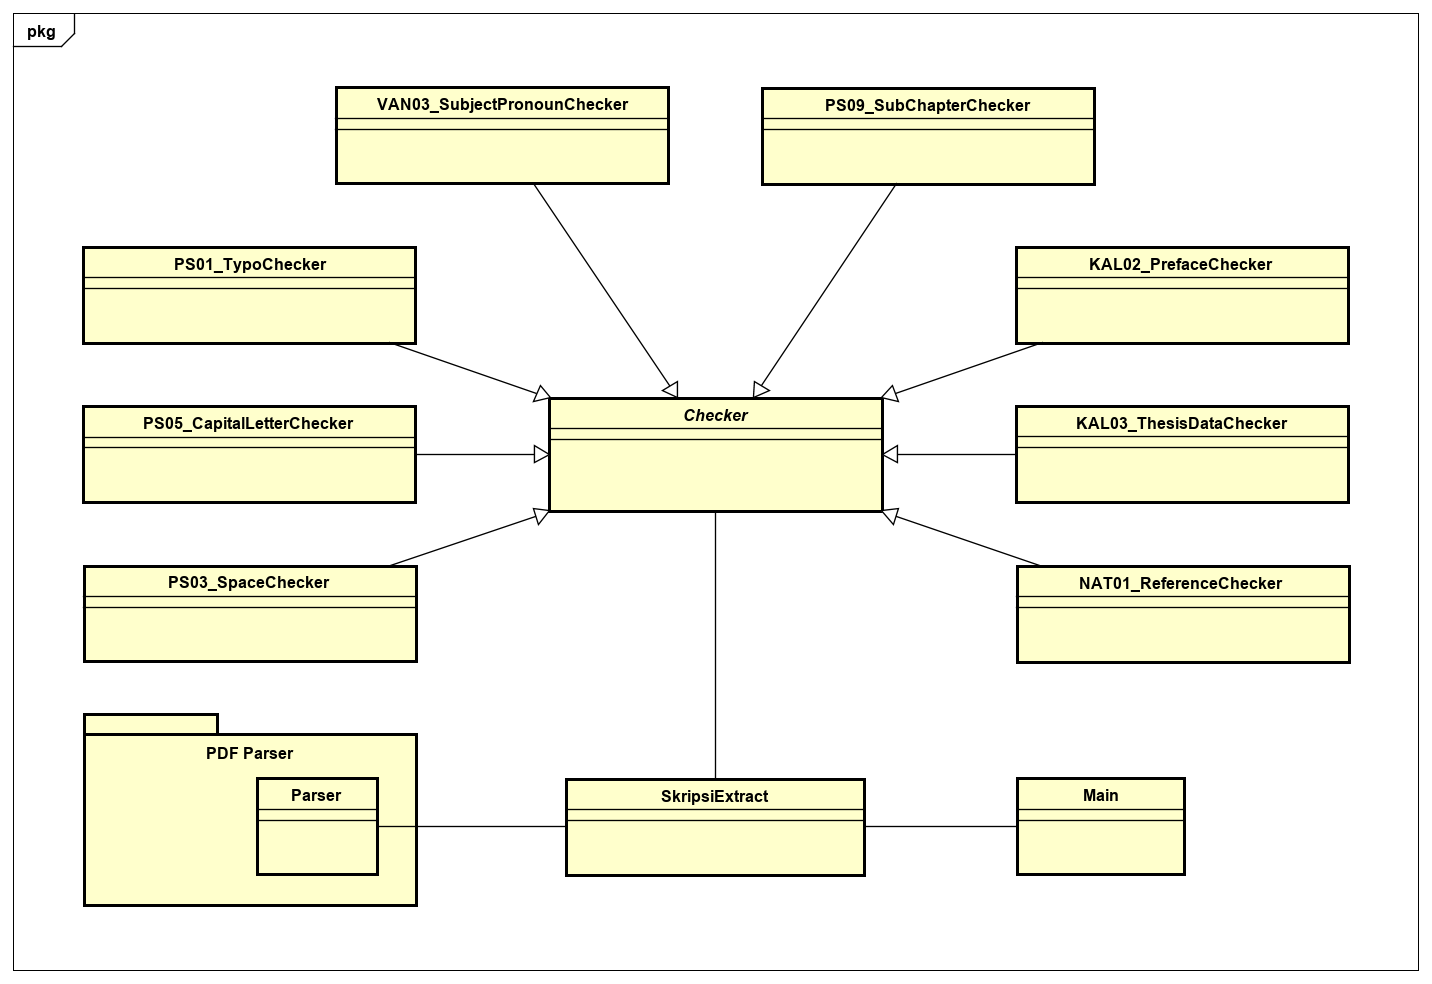
\includegraphics[scale=0.44]{class-diagram-kosong.png}
	\caption{Diagram kelas yang disederhanakan}	
	\label{fig:diagram_kelas} 
\end{figure}

Gambar \ref{fig:diagram_kelas} merupakan diagram kelas aplikasi pemeriksa kesalahan dokumen skripsi Informatika UNPAR yang telah disederhanakan. Pada diagram kelas tersebut, ditunjukan bahwa perangkat lunak memiliki sebelas kelas dan sebuah package \textit{library PDF Parser}. Terdapat sebuah kelas abstrak yang menjadi kelas \textit{parent} dari ke-8 fitur yang akan diimplementasikan dalam perangkat lunak. Delapan fitur yang ada akan memiliki method yang sama, namun berbeda proses pemeriksaanya. Rincian dari setiap kelas tersebut akan dijelaskan sebagai berikut.

\begin{enumerate}

	\item Kelas Checker \\
	
	\begin{figure}[H]
	\centering	
	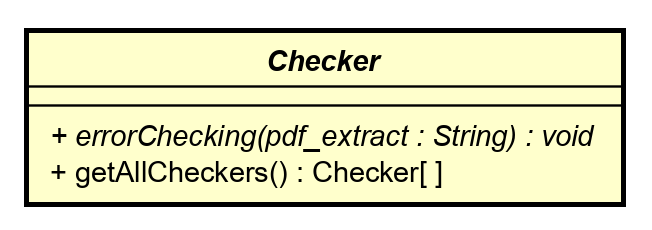
\includegraphics[scale=0.6]{checker.png}
	\caption{Kelas Checker}	
	\label{fig:checker} 
	\end{figure}

	Kelas ini merupakan kelas \textit{Parent} dari semua \textit{checker} yang akan diimplementasi pada perangkat lunak. Kelas ini memiliki sebuah \textit{method} abstrak dan sebuah \textit{method getter}, seperti yang ditunjukan pada Gambar \ref{fig:checker}. Semua anak kelas \textit{Checker} akan mengadopsi method yang ada pada kelas ini. Berikut ini adalah \textit{method} yang terdapat pada kelas \textit{Checker}.
	
		\begin{itemize}
			\item errorChecking(\$pdf\_extract) \\
			Method ini merupakan method abstrak, yang akan diturunkan kepada seluruh anak kelasnya. Method ini berfungsi untuk memeriksa kesalahan pada dokumen skripsi sesuai dengan peran yang diberikan pada kelas tersebut. Method ini menerima masukan pdf\_extract dengan tipe data kelas \textit{SkripsiExtract}. Parameter tersebut dapat digunakan oleh masing-masing kelas \textit{Checker} untuk memanggil \textit{method getter} yang diperlukan. Tidak semua pemeriksa memerlukan seluruh isi halaman dari dokumen skripsi. Sehingga proses pemeriksaan menjadi lebih efektif.		
			
			\item getAllChecker() \\
			Method ini berfungsi untuk melakukan instansiasi seluruh anak kelas \textit{Checker}. Method ini mengembalikan hasil instansiasi dari anak kelas \textit{Checker}. Hal ini akan mempermudah saat akan memanggil \textit{method errorChecking} pada setiap \textit{Checker} yang diimplementasi.
		\end{itemize}
	
	\item Kelas KAL02\_PrefaceChecker \\
	
	\begin{figure}[H]
	\centering	
	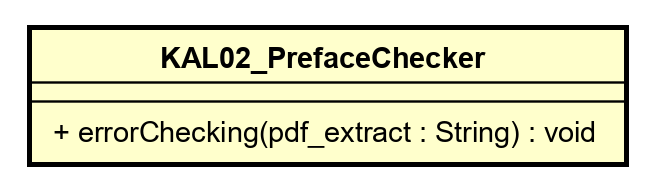
\includegraphics[scale=0.6]{kal02.png}
	\caption{Kelas KAL02\_PrefaceChecker}	
	\label{fig:kal02} 
	\end{figure}
	
	Kelas ini bertanggungjawab untuk memeriksa ada atau tidaknya kata pengantar sebelum memulai bab. Kelas ini memiliki sebuah method, yaitu errorChecking(\$pdf\_extract), seperti yang ditunjukan pada Gambar \ref{fig:kal02}. Method ini berfungsi untuk memeriksa kesalahan pada dokumen skripsi. Method ini menerima masukan pdf\_extract dengan tipe data kelas \textit{SkripsiExtract}. Bagian yang diperiksa pada \textit{checker} ini hanya bab 1 hingga 6.
	
	\item Kelas KAL03\_ThesisDataChecker \\
	
	\begin{figure}[H]
	\centering	
	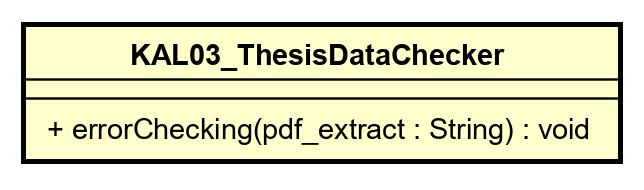
\includegraphics[scale=0.6]{kal03.png}
	\caption{Kelas KAL03\_ThesisDataChecker}	
	\label{fig:kal03} 
	\end{figure}
	
	Kelas ini bertanggungjawab untuk memeriksa kelengkapan data skripsi yang ditulis dalam bahasa Indonesia maupun bahasa Inggris. Dokumen skripsi akan menampilkan tulisan dari \textit{template} dokumen skripsi, apabila data skripsi belum diisi. Kelas ini memiliki sebuah \textit{method}, yaitu errorChecking(\$pdf\_extract). \textit{Method} ini berfungsi untuk memeriksa kesalahan pada dokumen skripsi. Method ini menerima masukan pdf\_extract dengan tipe data kelas \textit{SkripsiExtract}. Bagian yang diperiksa pada \textit{checker} ini adalah halaman cover bahasa Indonesia dan bahasa Inggris.
		
	\item Kelas NAT01\_ReferenceChecker \\
	
	\begin{figure}[H]
	\centering	
	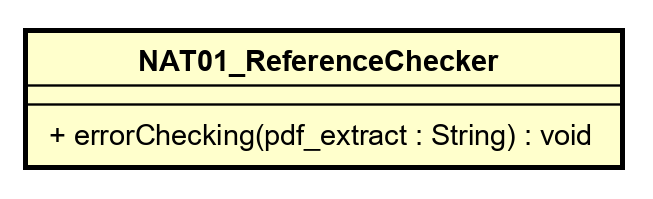
\includegraphics[scale=0.6]{nat01.png}
	\caption{Kelas NAT01\_ReferenceChecker}	
	\label{fig:nat01} 
	\end{figure}
	
	Kelas ini bertanggungjawab untuk memeriksa referensi yang akan dirujuk dalam dokumen. elas ini memiliki sebuah \textit{method}, yaitu errorChecking(\$pdf\_extract), seperti yang ditunjukan pada Gambar \ref{fig:nat01}. \textit{Method} ini berfungsi untuk memeriksa kesalahan pada dokumen skripsi. Method ini menerima masukan pdf\_extract dengan tipe data kelas \textit{SkripsiExtract}. Bagian yang diperiksa pada \textit{checker} ini adalah bab 1 hingga 6.
		
	\item Kelas PS01\_TypoChecker \\
	
	\begin{figure}[H]
	\centering	
	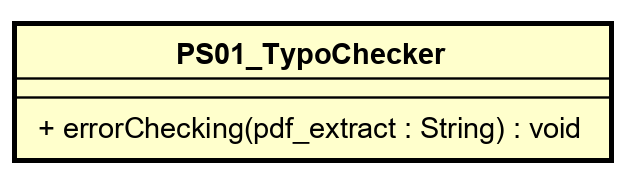
\includegraphics[scale=0.6]{ps01.png}
	\caption{Kelas PS01\_TypoChecker}	
	\label{fig:ps01} 
	\end{figure}
	
	Kelas ini bertanggungjawab untuk memeriksa kesalahan penulisan kata. Kelas ini memiliki sebuah method, yaitu errorChecking(\$pdf\_extract), seperti yang ditunjukan pada Gambar \ref{fig:ps01}. \textit{Method} ini berfungsi untuk memeriksa kesalahan pada dokumen skripsi. Method ini menerima masukan pdf\_extract dengan tipe data kelas \textit{SkripsiExtract}. Bagian yang diperiksa pada \textit{checker} ini adalah bab 1 hingga 6.
			
	\item Kelas PS03\_SpaceChecker \\
	
	\begin{figure}[H]
	\centering	
	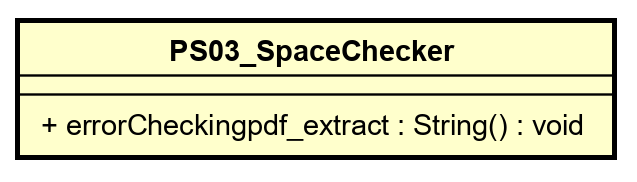
\includegraphics[scale=0.6]{ps03.png}
	\caption{Kelas PS03\_SpaceChecker}	
	\label{fig:ps03} 
	\end{figure}	
		
	Kelas ini bertanggungjawab untuk memeriksa penggunaan spasi sebelum dan setelah tanda baca. Kelas ini memiliki sebuah method, yaitu errorChecking(\$pdf\_extract), seperti yang ditunjukan pada Gambar \ref{fig:ps03}. \textit{Method} ini berfungsi untuk memeriksa kesalahan pada dokumen skripsi. Method ini menerima masukan pdf\_extract dengan tipe data kelas \textit{SkripsiExtract}. Bagian yang diperiksa pada \textit{checker} ini adalah bab 1 hingga 6.
			
	\item Kelas PS05\_CapitalLetterChecker \\
	
	\begin{figure}[H]
	\centering	
	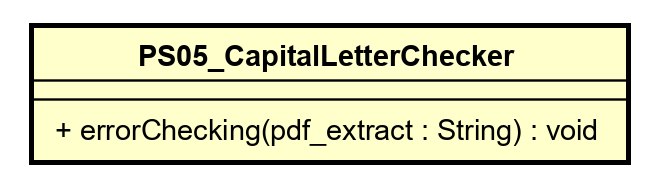
\includegraphics[scale=0.6]{ps05.png}
	\caption{Kelas PS05\_CapitalLetterChecker}	
	\label{fig:ps05} 
	\end{figure}
	
	Kelas ini bertanggungjawab untuk memeriksa penggunaan huruf kapital pada awal kalimat. Kelas ini memiliki sebuah method, yaitu errorChecking(\$pdf\_extract), seperti yang ditunjukan pada Gambar \ref{fig:ps05}. \textit{Method} ini berfungsi untuk memeriksa kesalahan pada dokumen skripsi. Method ini menerima masukan pdf\_extract dengan tipe data kelas \textit{SkripsiExtract}. Bagian yang diperiksa pada \textit{checker} ini adalah bab 1 hingga 6.
			
	\item Kelas PS09\_SubChapterChecker \\

	\begin{figure}[H]
	\centering	
	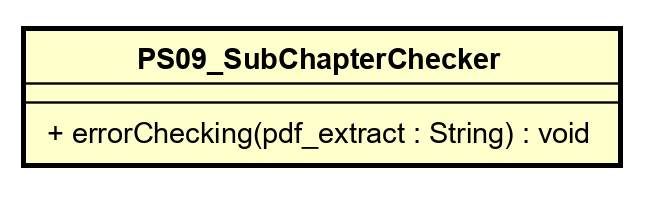
\includegraphics[scale=0.6]{ps09.png}
	\caption{Kelas PS09\_SubChapterChecker}	
	\label{fig:ps09} 
	\end{figure}	
	
	Kelas ini bertanggungjawab untuk memeriksa jumlah sub bab atau sub sub bab yang ada dalam sebuah bab atau sub bab. Kelas ini memiliki sebuah method, yaitu errorChecking(\$pdf\_extract), seperti yang ditunjukan pada Gambar \ref{fig:ps09}. \textit{Method} ini berfungsi untuk memeriksa kesalahan pada dokumen skripsi. Method ini menerima masukan pdf\_extract dengan tipe data kelas \textit{SkripsiExtract}. Bagian yang diperiksa pada \textit{checker} ini adalah halaman daftar isi.
			
	\item Kelas VAN03\_SubjectProunounChecker \\
	
	\begin{figure}[H]
	\centering	
	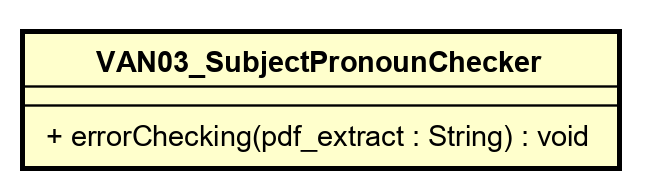
\includegraphics[scale=0.6]{van03.png}
	\caption{Kelas VAN03\_SubjectProunounChecker}	
	\label{fig:van03} 
	\end{figure}
	
	Kelas ini bertanggungjawab untuk memeriksa penggunaan kata ganti orang pada dokumen skripsi. Kelas ini memiliki sebuah method, yaitu errorChecking(\$pdf\_extract), seperti yang ditunjukan pada Gambar \ref{fig:van03}. \textit{Method} ini berfungsi untuk memeriksa kesalahan pada dokumen skripsi. Method ini menerima masukan pdf\_extract dengan tipe data kelas \textit{SkripsiExtract}. Bagian yang diperiksa pada \textit{checker} ini adalah bab 1 hingga 6.
			
	\item Kelas SkripsiExtract \\
	
	\begin{figure}[H]
	\centering	
	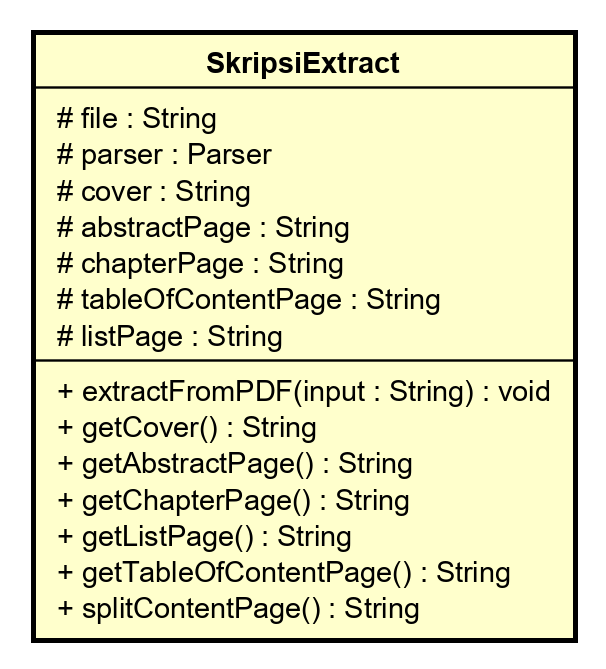
\includegraphics[scale=0.6]{skripsi_extract.png}
	\caption{Kelas SkripsiExtract}	
	\label{fig:skripsiExtract} 
	\end{figure}
	
	Kelas ini berfungsi untuk melakukan proses ekstak dokumen PDF skripsi, dengan menggunakan \textit{library PdfParser}. Hasil dari ekstrak tersebut akan disimpan menjadi beberapa bagian, berdasarkan konten-konten yang ada pada dokumen skripsi. Kelas ini memiliki beberapa atribut yang akan dijelaskan sebagai berikut:
	
		\begin{itemize}
			\item file \\
			Atribut ini berfungsi untuk menyimpan lokasi dokumen skripsi beserta nama dari dokumen tersebut.
			
			\item parser \\			
			Atribut ini berfungsi sebagai instansiasi kelas Parser dari \textit{Library PDF Parser}, untuk memanggil method yang dibutuhkan dalam proses ekstrak dokumen.
			
			\item cover \\
			Atribut ini berfungsi untuk menyimpan hasil ekstrak dari halaman cover bahasa Indonesia dan bahasa Inggris.
			
			\item abstractPage \\			
			Atribut ini berfungsi untuk menyimpan hasil ekstrak dari halaman abstrak bahasa Indonesia dan bahasa Inggris.
			
			\item otherPage \\
			Atribut ini berfungsi untuk menyimpan hasil ekstrak dari halaman lembar pengesahan, pernyataan dan kata pengantar.
			
			\item tableOfContentPage \\
			Atribut ini berfungsi untuk menyimpan hasil ekstrak dari halaman daftar isi.
			
			\item contentPage \\	
			Atribut ini berfungsi untuk menyimpan hasil ekstrak mulai dari bab 1 hingga bab 6.
			
			\item listPage \\
			Atribut ini berfungsi untuk menyimpan hasil ekstrak pada halaman daftar tabel, daftar gambar, daftar referensi dan lampiran.
			
		\end{itemize}
	
	Kelas ini juga memiliki \textit{method} yang berkaitan dengan proses ekstrak dokumen skripsi dan penyimpanan hasil ekstraknya. Berikut adalah \textit{method} yang terdapat pada kelas ini:
		
		\begin{itemize}
			\item extractFromPDF(\$input) \\
			Method ini berfungsi untuk melakukan proses ekstrak file PDF skripsi. Hasil dari ekstrak tersebut akan disimpan ke dalam beberapa bagian, seperti cover, halaman abstrak, dan sebagainya. 
			
			\item getCoverPage() \\
			Method ini berfungsi untuk mendapatkan halaman cover skripsi dalam bahasa Indonesia dan bahasa Inggris.
			
			\item getAbstractPage() \\
			Method ini berfungsi untuk mendapatkan halaman abstrak dalam bahasa Indonesia dan bahasa Inggris.
			
			\item getOtherPage() \\
			Method ini berfungsi untuk mendapatkan halaman lembar pengesahan, pernyataan dan kata pengantar.
			
			\item getTableOfContentPage() \\
			Method ini berfungsi untuk mendapatkan halaman daftar isi. Method ini akan menyaring sub bab dan sub sub bab yang terdapat pada daftar isi.
			
			\item getListPage() \\
			Method ini berfungsi untuk mendapatkan halaman daftar gambar, daftar tabel dan daftar referensi.
			
			\item getContentPage() \\
			Method ini berfungsi untuk mendapatkan halaman konten skripsi dari bab 1 sampai 6.
			
			\item splitContentPage() \\
			Method ini memiliki fungsi yang hampir sama dengan method \textit{getContentPage}, yaitu untuk mendapatkan halaman konten skripsi. Namun, pada method ini ada beberapa proses pemisahan isi konten (per kalimat) ke dalam beberapa array. Fitur-fitur dalam perangkat lunak yang memerlukan pemeriksaan berdasarkan kalimat dapat langsung memanggil method ini. 
			
		\end{itemize}
	
	\item Kelas Main \\
	Kelas ini digunakan untuk menjalankan perangkat lunak. Kelas ini tidak memiliki atribut dan \textit{method}, hanya terdiri dari beberapa baris kode yang memanggil \textit{method} untuk mengekstrak dan memeriksa file PDF skripsi. 

\end{enumerate} 

\section{Perancangan Algoritma}
Pada bagian ini akan dijelaskan perancangan algoritma untuk mengekstrak dokumen skripsi dan pola pengecekan kesalahan yang akan digunakan pada perangkat lunak.
 
\subsection{Algoritma untuk Mengekstrak Dokumen}
Dokumen skripsi yang dapat diperiksa dalam perangkat lunak merupakan dokumen skripsi Teknik Informatika Unpar, yang memiliki ekstensi \textit{PDF}. Sebelum dilakukan pemeriksaan kesalahan, dokumen tersebut perlu diekstrak terlebih dulu. Pada skripsi ini, aplikasi akan menggunakan \textit{library PDFParser} untuk mengekstrak dokumen skripsi. Pada \textit{library} tersebut, terdapat 2 metode yang dapat digunakan untuk mengekstrak dokumen. Penjelasan dari ke-2 metode tersebut akan diuraikan pada sebagai berikut.
	
\begin{lstlisting}[caption={Potongan kode untuk mengesktrak seluruh halaman dokumen}	\label{lst:all_page},language=php,xleftmargin=.2\textwidth] 
include 'vendor/autoload.php';
	
$parser = new \Smalot\PdfParser\Parser();
$pdf    = $parser->parseFile('document.pdf');
$text   = $pdf->getText();
\end{lstlisting}
\medskip
	
\begin{lstlisting}[caption={Potongan kode untuk mengesktrak halaman dokumen secara spesifik}
\label{lst:specific_page},language=php,xleftmargin=.2\textwidth] 
include 'vendor/autoload.php';

$parser = new \Smalot\PdfParser\Parser();
$pdf    = $parser->parseFile('document.pdf');
$pages  = $pdf->getPages();
\end{lstlisting}
\medskip

Listing \ref{lst:all_page} dan Listing \ref{lst:specific_page} merupakan potongan kode yang terdapat pada dokumentasi \textit{library PDF Parser}, yang digunakan untuk mengekstrak isi dokumen. Kode dari kedua listing tersebut hampir mirip, yang menjadi pembeda adalah pada baris ke-5. Listing \ref{lst:all_page} menggunakan \textit{method getText()} dan hasil dari ekstraknya disimpan menjadi sebuah kesatuan dari halaman awal hingga halaman akhir. Listing \ref{lst:specific_page} menggunakan \textit{method getPages()} dan hasil dari ekstraknya disimpan dalam sebuah array String sejumlah halaman yang ada pada dokumen. Pengguna dapat menentukan secara spesifik halaman apa saja yang ingin diekstrak.

Pada skripsi ini akan digunakan metode yang mengesktrak halaman-halaman secara spesifik. Hasil ekstrak akan disimpan dalam berdasarkan konten-konten yang ada, seperti halaman cover, abstrak, daftar isi, daftar tabel, daftar gambar dan seterusnya. Ada beberapa alasan yang mendorong untuk melakukan pemisahan konten-konten tersebut, salah satunya yaitu agar pemeriksa dapat memeriksa bagian-bagian spesifik yang dibutuhkan. Contohnya, untuk memeriksa kelengkapan data skripsi tidak perlu memeriksa seluruh isi dari dokumen, halaman yang dibutuhkan hanya cover saja. Dengan demikian, proses pemeriksaan menjadi lebih efektif karena tidak perlu memeriksa seluruh halaman yang ada pada dokumen.

\subsection{Algoritma Pemeriksa Kesalahan}
Hasil survei kesalahan-kesalahan dalam penulisan dokumen skripsi sudah disaring dan akan diimplementasikan dalam perangkat lunak. Pengecekan kesalahan tersebut akan dilakukan dengan menggunakan teknik \textit{pattern matching}. Hasil ekstrak dari PDF skripsi akan dipotong per kalimat dengan \textit{delimiter} karakter titik dan spasi ke dalam sebuah array. Berikut adalah rincian dari hasil survei yang dipilih beserta penyelesaiannya:

\begin{enumerate}
	\item Penulisan kata (PS-01) \\
	Untuk mendeteksi kesalahan penulisan kata, akan digunakan ekstensi kamus bahasa Indonesia \textit{LibreOffice}. Dengan digunakannya kamus tersebut, kesalahan penulisan suatu kata dapat diminimalisir. Pada skripsi ini, pemeriksaan kata-kata yang menggunakan imbuhan tidak ditangani pada masalah ini, karena keterbatasan waktu yang dimiliki. Terdapat kode yang harus diterjemahkan terlebih dahulu untuk dapat mengetahui imbuhan yang dapat digunakan dalam sebuah kata, seperti yang sudah dijelaskan pada sub bab \ref{sec:kamusindo}. Pola pengecekan yang digunakan akan dijelaskan pada Pseudocode \ref{alg:ps01}.
		
\begin{minipage}{1.0\linewidth}
\begin{algorithm}[H]
    \caption{Typo checker function}
	\label{alg:ps01}
	\begin{algorithmic}[1]
		\State Input: An object from the SkripsiExtract class to call the getter method
		\State Output: An array containing error reports    	
		\State
    	\Function{ErrorChecking}{\$pdf\_exctract}
    		\State $temp \gets$ Split dictionary based on newline
			\State $dictionary \gets$ Array for store dictionary
			\For{$i = 0$ to size of temp}
				\State Remove affix code from each index dictionary array 
			\EndFor
			\State $word \gets$ Call getter from class SkripsiExtract and split with non word character
			\State $typos \gets$ Array for store typos
			\For{each word in $array$}
        		\If{$value$ not contain in $dictionary$ and $value$ not contain in $typos$}
                	\State Fill $typos$ with $value$
            	\EndIf
        	\EndFor
			\State $result \gets$ Array for store all errors report
    		\If{size of $typos$ greater than 0}
                \State $result \gets$ Add all errors report into $result$
            \EndIf
    		\State \textbf{return} $result$
    	\EndFunction
	\end{algorithmic}
\end{algorithm}
\end{minipage}
\medskip

	Pada Pseudocode \ref{alg:ps01}, pola akan memeriksa setiap kata yang ada pada indeks array. Namun untuk pemeriksaan kata ini hanya untuk kata yang menggunakan bahasa Indonesia saja. Pola akan mencocokan kata yang akan diperiksa dengan kamus bahasa Indonesia \textit{LibreOffice}. Berikut adalah contoh dari kesalahan dan laporan yang dikeluarkan:
	
	\begin{itemize}
		\item Contoh kesalahan \\
		Istilah \textit{regex} berasal dari toeri matematika dan komputer sains, yang mencerminkan sifat ekspresi dalam matematika yang disebut keteraturan.
		\item Laporan kesalahan \\
		Pada fitur ini, setiap menemukan kesalahan penulisan kata akan ditampung terlebih dahulu sampai seluruh kata selesai diperiksa. Pada akhirnya seluruh kesalahan yang ditemukan akan dikeluarkan.
	\end{itemize}
	
	\item Pemberian spasi sesudah tanda baca (PS-03) \\
	Kesalahan ini akan terdeteksi apabila tidak ada karakter spasi sesudah tanda baca. Pola pengecekan yang digunakan akan dijelaskan pada \textit{pseudocode} \ref{alg:ps03}.
	
\begin{minipage}{1.0\linewidth}
\begin{algorithm}[H]
    \caption{Space checker function}
	\label{alg:ps03}
	\begin{algorithmic}[1]
		\State Input: An object from the SkripsiExtract class to call the getter method
		\State Output: An array containing error reports
		\State
    	\Function{ErrorChecking}{\$pdf\_exctract}
			\State $result \gets$ Array for store all errors report
			\State $sentence \gets$ Call getter from class SkripsiExtract
    		\For{each sentence in $sentence$}
				\State $pattern \gets$ Define regex /([A-Za-z]$\lbrace$2,$\rbrace$[,.!?][A-Za-z]+)/
        		\If{$pattern$ contain in $array$}
                	\State $result \gets$ Fill with errors report
            	\EndIf
        	\EndFor
    		\State \textbf{return} $result$
    	\EndFunction
	\end{algorithmic}
\end{algorithm}
\end{minipage}
\medskip
	
	Pada Pseudocode \ref{alg:ps03}, pola akan memeriksa setiap kalimat yang ada pada indeks array. Pola \textit{regex} yang telah didefinisikan akan mencari pola yang apabila setelah tanda baca titik, koma, seru atau tanya tidak terdapat spasi yang memisahkan tanda baca dengan kata setelah tanda baca. Berikut adalah contoh dari kesalahan dan laporan yang dikeluarkan:
	
	\begin{itemize}
		\item Contoh kesalahan \\
		Aplikasi ini dijalankan melalui melalui terminal command Windows.laporan dari hasil kesalahan tersebut akan ditampilkan melalui terminal command Windows.
		\item Laporan kesalahan \\
		Perhatikan spasi setelah tanda baca.
	\end{itemize}
	
	\item Awal kalimat tidak menggunakan huruf kapital (PS-05) \\
	Kesalahan ini akan terdeteksi apabila setelah tanda baca pada akhir kalimat, karakter pertama setelah spasi menggunakan huruf kecil. Pola pengecekan yang digunakan akan dijelaskan pada \textit{pseudocode} \ref{alg:ps05}.

\begin{minipage}{1.0\linewidth}
\begin{algorithm}[H]
    \caption{Capital letter checker function}
	\label{alg:ps05}
	\begin{algorithmic}[1]
		\State Input: An object from the SkripsiExtract class to call the getter method
		\State Output: An array containing error reports	    	
    	\Function{ErrorChecking}{\$pdf\_exctract}
    		\State $result \gets$ Array for store all errors report
			\State $sentence \gets$ Call getter from class SkripsiExtract
			\State    		
    		\For{each sentence in $sentence$}
				\State $pattern \gets$ Define regex / $\hat{}$ [a-z]+ | [a-z]+$\backslash$.[a-z] /
        		\If{$pattern$ contain in $array$}
        			\If{first character in a sentence is a non word character}
        				\State Continue
        			\EndIf{}
        			\Else
                		\State $result \gets$ Fill with errors report
            	\EndIf
        	\EndFor
    		\State \textbf{return} $result$
    	\EndFunction
	\end{algorithmic}
\end{algorithm}
\end{minipage}
\medskip

	Pada Pseudocode \ref{alg:ps05}, pola akan memeriksa setiap kalimat yang ada pada indeks array. Pola \textit{regex} yang telah didefinisikan akan mencari pola dimana karakter pertama dalam sebuah kalimat menggunakan huruf kecil. Namun perlu dipastikan bahwa karakter pertama tersebut adalah karakter \textit{word}.Berikut adalah contoh dari kesalahan dan laporan yang dikeluarkan:
	
	\begin{itemize}
		\item Contoh kesalahan \\ 
		aplikasi sederhana ini, dapat dimanfaatkan oleh mahasiswa Informatika Unpar secara mandiri.
		\item Laporan kesalahan \\
		Huruf pertama pada kalimat ini tidak menggunakan huruf kapital
	\end{itemize}
	
	\item Jumlah subbab dalam 1 bab tidak boleh hanya 1 (PS-09) \\
	Kesalahan ini dapat diselesaikan dengan mencari jumlah subbab yang ada dalam sebuah bab. Pola pengecekan yang digunakan akan dijelaskan pada \textit{pseudocode} \ref{alg:ps09}.

\begin{minipage}{1.0\linewidth}
\begin{algorithm}[H]
    \caption{Subchapter checker function}
	\label{alg:ps09}
	\begin{algorithmic}[1]
		\State Input: An object from the SkripsiExtract class to call the getter method
		\State Output: An array containing error reports 
		\State   	
    	\Function{ErrorChecking}{\$pdf\_exctract}
    		\State $result \gets$ Array for store all errors report
			\State $sentence \gets$ Call getter from class SkripsiExtract
			\State $array \gets$ Merge an empty array with $temp$
    		\For{$i \gets$ 0 to size of $array$ }
				if($array[$i$]$ contains ''.1'')				
				\State $substring \gets$ get substring element from index $i+1$ (substring from 0 to length of $array[$i$]-1$)
        		\If{$array$ not contain $substring$ append with 2}
                	\State fill $result$ with errors report
            	\EndIf
        	\EndFor
    		\State \textbf{return} $result$
    	\EndFunction
	\end{algorithmic}
\end{algorithm}
\end{minipage}
\medskip
	
	Pada Pseudocode \ref{alg:ps09}, pola akan memeriksa setiap kalimat yang ada pada indeks array. Kesalahan akan terdeteksi apabila karakter pertama dalam sebuah kalimat menggunakan huruf kecil. Berikut adalah contoh dari kesalahan dan laporan yang dikeluarkan:
	
	\begin{itemize}
		\item Contoh kesalahan \\
		Bab 4 \newline PERANCANGAN \newline \newline 4.1 Perancangan Kelas
		\item Laporan kesalahan \\
		Bab/Sub bab .... ini hanya terdapat 1 sub bab/sub sub bab.
	\end{itemize}	
	
	\item Kalimat pengantar untuk setiap subbab (KAL-02) \\
	Kesalahan ini dapat dideteksi dengan melihat ada atau tidaknya kalimat setelah subbab dibuat. Pola pengecekan yang digunakan akan dijelaskan pada \textit{pseudocode} \ref{alg:kal02}.

\begin{minipage}{1.0\linewidth}
\begin{algorithm}[H]
    \caption{Preface checker function}
	\label{alg:kal02}
	\begin{algorithmic}[1]
		\State Input: An object from the SkripsiExtract class to call the getter method
		\State Output: An array containing error reports    
		\State	
    	\Function{ErrorChecking}{\$pdf\_exctract}
    		\State $result \gets$ Array for store all errors report
			\State $sentence \gets$ Call getter from class SkripsiExtract
    		\For{each sentence in $sentence$}
				\State $pattern \gets$ Define regex / $\hat{}$ (BAB )[0-9]$\lbrace$1$\rbrace$[$\backslash$sA-Z]$\lbrace$ $\rbrace$1,[0-9]+ /
        		\If{$pattern$ contain in $array$}
                	\State fill $result$ with errors report
            	\EndIf
        	\EndFor
    		\State \textbf{return} $result$
    	\EndFunction
	\end{algorithmic}
\end{algorithm}
\end{minipage}
\medskip

	Pada pseudocode \ref{alg:kal02}, pola akan memeriksa setiap kalimat yang ada pada indeks array. Kesalahan akan terdeteksi apabila tidak terdapat kalimat yang mengawali bab tersebut. Berikut adalah contoh dari kesalahan dan laporan yang dikeluarkan:
	
	\begin{itemize}
		\item Contoh kesalahan \\
		Bab 4 \newline PERANCANGAN \newline \newline 4.1 Perancangan Kelas \newline 4.2 Perancangan Algoritma
		\item Laporan kesalahan \\
		Berilah kata pengantar untuk setiap bab.
	\end{itemize}
	
	\item Kelengkapan data skripsi (KAL-03) \\
	Kesalahan ini dapat terlihat pada halaman cover skripsi. Pada halaman cover bahasa Inggris dan bahasa Indonesia akan ditemukan tulisan \textit{template}, apabila mahasiswa belum mengisi data skripsi. Data tersebut diisi pada file ''Data.tex''. Pola pengecekan yang digunakan akan dijelaskan pada \textit{pseudocode} \ref{alg:kal03}.
	
\begin{minipage}{1.0\linewidth}
\begin{algorithm}[H]
    \caption{Thesis data checker function}
	\label{alg:kal03}
	\begin{algorithmic}[1]
		\State Input: An object from the SkripsiExtract class to call the getter method
		\State Output: An array containing error reports  
		\State  	
    	\Function{ErrorChecking}{\$pdf\_exctract}
    		\State $result \gets$ Array for store all errors report
			\State $sentence \gets$ Call getter from class SkripsiExtract
    		\For{each sentence in $sentence$}
				\State $pattern \gets$ Define regex /$\backslash$bJUDUL BAHASA INDONESIA$\backslash$b|$\backslash$bJUDUL BAHASA INGGRIS$\backslash$b|$\backslash$bNama Lengkap$\backslash$b|$\backslash$b10 digit NPM UNPAR$\backslash$b|$\backslash$btahun$\backslash$b/
        		\If{$pattern$ contain in $array$}
                	\State fill $result$ with errors report
            	\EndIf
        	\EndFor
    		\State \textbf{return} $result$
    	\EndFunction
	\end{algorithmic}
\end{algorithm}
\end{minipage}	
\medskip
	
	Pada Pseudocode \ref{alg:kal03}, pola akan memeriksa halaman cover bahasa Indonesia dan bahasa Inggris. Kesalahan akan terdeteksi pada halaman cover masih terdapat kalimat yang terdapat dalam template. Berikut adalah contoh dari kesalahan dan laporan yang dikeluarkan:
	
	\begin{itemize}
		\item Contoh kesalahan \\
		<<SKRIPSI/TUGAS AKHIR>> \newline <<Judul Bahasa Indonesia>> \newline Marcell Trixie Alexander \newline <<10 digit NPM UNPAR>>
		\item Laporan kesalahan \\
		Ada data skripsi yang belum dilengkapi pada halaman cover.
	\end{itemize}	
	
	\item Penggunaan kata ganti orang (VAN-03) \\
	Kesalahan ini dapat diatasi dengan memasukan kata-kata yang termasuk dalam kata ganti orang menjadi kata-kata yang tidak dapat digunakan. Pola pengecekan yang digunakan akan dijelaskan pada \textit{pseudocode} \ref{alg:van03}.

\begin{minipage}{1.0\linewidth}
\begin{algorithm}[H]
    \caption{Subject Pronoun checker function}
	\label{alg:van03}
	\begin{algorithmic}[1]
		\State Input: An object from the SkripsiExtract class to call the getter method
		\State Output: An array containing error reports
		\State
    	\Function{ErrorChecking}{\$pdf\_exctract}
			\State $result \gets$ Array for store all errors report
			\State $sentence \gets$ Split PDF parsing results based on dots and space
    		\For{each sentence in $sentence$}
				\State $pattern \gets$ Define regex /$\backslash$bsaya$\backslash$b | $\backslash$bkamu$\backslash$b | $\backslash$bdia$\backslash$b/i/
        		\If{$pattern$ contain in $array$}
                	\State fill $result$ with errors report
            	\EndIf
        	\EndFor
    		\State \textbf{return} $result$
    	\EndFunction
	\end{algorithmic}
\end{algorithm}
\end{minipage}
\medskip

	Pada Pseudocode \ref{alg:van03}, pola akan memeriksa setiap kalimat yang ada pada indeks array. Kesalahan akan terdeteksi pada kalimat terdapat kata ganti orang. Berikut adalah contoh dari kesalahan dan laporan yang dikeluarkan:
	
	\begin{itemize}
		\item Contoh kesalahan \\
		Saya akan membuat aplikasi ini menggunakan bahasa pemrograman PHP.
		\item Laporan kesalahan \\
		Kalimat ini mengandung kata ganti orang.
	\end{itemize}	
	
	\item Penulisan daftar referensi (NAT-01) \\
	Kesalahan dalam penulisan daftar referensi dapat dilihat dengan munculnya tanda ''[?]'', yang menandakan bahwa referensi tersebut tidak dirujuk dengan baik. Pola pengecekan yang digunakan akan dijelaskan pada \textit{pseudocode} \ref{alg:nat01}.

\begin{minipage}{1.0\linewidth}
\begin{algorithm}[H]
    \caption{Reference checker function}
	\label{alg:nat01}
	\begin{algorithmic}[1]
		\State Input: An object from the SkripsiExtract class to call the getter method
		\State Output: An array containing error reports
		\State
    	\Function{ErrorChecking}{\$pdf\_exctract}
			\State $result \gets$ Array for store all errors report
			\State $sentence \gets$ Call getter from class SkripsiExtract
    		\For{each sentence in $sentence$}
				\State $pattern \gets$ Define regex /$\backslash$B$\backslash$[ $\backslash$?$\backslash$]$\backslash$B/
        		\If{$pattern$ contain in $array$}
                	\State fill $result$ with errors report
            	\EndIf
        	\EndFor
    		\State \textbf{return} $result$
    	\EndFunction
	\end{algorithmic}
\end{algorithm}
\end{minipage}
\medskip

	Pada Pseudocode \ref{alg:nat01}, pola akan memeriksa setiap kalimat yang ada pada indeks array. Kesalahan akan terdeteksi kalimat terdapat simbol ''[?]'', yang menandakan referensi tidak dirujuk dengan baik. Berikut adalah contoh dari kesalahan dan laporan yang dikeluarkan:
	
	\begin{itemize}
		\item Contoh kesalahan \\
		\textit{Regular expression} [?] adalah jenis pola teks tertentu yang dapat digunakan pada banyak aplikasi modern dan bahasa pemrograman.
		\item Laporan kesalahan \\
		Referensi tidak dirujuk dengan baik, lakukan perintah PDFLatex->BibTex->PDFLatex->PDFLatex untuk memperbaikinya.
	\end{itemize}		
	
\end{enumerate}